\documentclass[12pt,letterpaper]{scrreprt}
\usepackage{subfigure}
\usepackage[latin1]{inputenc}
\usepackage{amsmath}
\usepackage{amsfonts}
\usepackage{amssymb}
\usepackage{graphicx}
\usepackage{todonotes}
\usepackage{appendix}
\usepackage{pdfpages}
\usepackage{lineno}
\usepackage{url}
\usepackage[colorlinks=true,linkcolor=blue,citecolor=blue,urlcolor=blue]{hyperref}

\linenumbers

\author{P. Bachant, M. Wosnik, B. Gunawan, V. Neary}
\title{Test Plan: UNH RM2 Tow Tank Experiment}

\begin{document}

\begin{titlepage}
    \centering
    \addtolength{\topmargin}{.5in}
    {\bfseries \large
        Experimental Test Plan: 1:6 Scale Reference Model 2 Cross-Flow Turbine
    }  
    \vskip1cm
    P. Bachant$^1$\\
    M. Wosnik$^1$\\
    B. Gunawan$^2$\\
    V. Neary$^2$\\  
    \vfill
    $^1$Center for Ocean Renewable Energy \\
    University of New Hampshire \\
    Durham, NH \\
    \vspace{0.1in}
    $^2$Water Power Technologies \\
    Sandia National Laboratories \\
    Albuquerque, NM \\
    \vfill
    December 15, 2014
    \vfill
    \textbf{Prepared by:}\\
    Center for Ocean Renewable Energy\\
    University of New Hampshire\\
    Durham, NH\\
    \vspace{0.1in}
    \textbf{Prepared for:} \\
    Wind and Water Power Technologies Program \\
    Office of Energy Efficiency and Renewable Energy \\
    U.S. Department of Energy \\
    Washington, D.C.
    \vfill
    
\includegraphics[width=0.32\textwidth]{Figures/unhlogo} \\
    \vspace{0.1in}
    
\includegraphics[width=0.41\textwidth]{Figures/snllogo} \\
    \vspace{0.1in}
    
\includegraphics[width=0.34\textwidth]{Figures/doelogo}
    \vfill
\end{titlepage}

\tableofcontents

\newpage
\listoftodos

\chapter{Introduction}

Sandia National Laboratory (SNL) developed the cross-flow turbine, Reference
Model 2 (RM2), to estimate the levelized cost of energy (LCOE), and to provide
open power performance data from scaled model testing that can be used to
validate open-source design tools.  More details on the reference modeling
effort are provided in Neary et al. \cite{Neary2014}.

Dimensional analysis provides scaling laws that are used to upscale model test
data into performance and design information for a full-scale prototype turbine.
For hydrokinetic turbines, hydrodynamic similitude is achieved when the chord
Reynolds number $Re$, Froude number $Fr$, and the tip speed ratio
$\lambda=\omega R/U_\infty$ of the model and the full-scale device are the same.
It is rare to achieve perfect similitude for $Re$, but a threshold value should
be exceeded, such that scale model results can be extrapolated. Note that in
this study we are focusing on $Re$, not $Fr$ as the dominant scaling parameter
since $Fr \ll 1$.

\todo[inline]{Get ref for ``Froude number similitude in tow tank testing is
important for upscaling wake flow data'' before adding above.}

As a cross-flow turbine, the RM2 blades will experience large variations in
angles of attack as they rotate about their axis (``cross-flow turbine'' means
the axis of rotation is perpendicular to flow direction---can be vertical or
horizontal). This range of angles of attack becomes larger as the tip speed
ratio decreases \cite{Para2002}. The variation is typically sufficiently large
that the blades operate under dynamic stall, which is a complex unsteady
process, deviating significantly from static foil behavior. Furthermore, the
higher the solidity of a cross-flow turbine, the lower the optimal tip-speed
ratio at which it operates. Marine Hydrokinetic (MHK) cross-flow turbines
typically have higher solidity than cross-flow wind turbines (VAWT), and hence
operate at lower tip-speed ratios. Since MHK turbines operate in a higher
density fluid, unsteady dynamic effects related to the blades' pitching motion
and flow curvature also become more important when compared to wind turbines.

The performance of cross-flow MHK turbines thus depends on both Reynolds number
and solidity (note that these issues are related, since an average blade chord
Reynolds number, $Re_{c,\mathrm{avg}} \approx \lambda U_\infty c/ \nu$, can be
expressed in terms of tip speed ratio, which is a function of solidity). If
numerical models are validated with physical model data that was obtained at
insufficiently high Reynolds numbers, it cannot be determined whether problems
with model predictions are caused by Reynolds number effects, issues related to
higher solidity, or both. It is uncertain whether numerical models validated
with physical model data obtained at low Reynolds number should be considered
validated at all, since the scale at which the model will be applied is orders
of magnitude larger. One way to overcome this uncertainty is to show that the
scaled physical model test has become Reynolds number independent, and therefore
validation efforts should be relevant at full-scale. 

For example, the effect of Reynolds number on average power output was shown to
be significant on the 2 m Sandia Research Darrieus turbine in wind tunnel
testing \cite{Blackwell1976}: Maximum power coefficient, $C_{P,\mathrm{max}}$,
increased with Reynolds number, $Re_c$, along with a shift of the location of
$C_{P,\mathrm{max}}$ toward lower tip speed ratios due to delayed blade stall.
The effects of Reynolds number were quite dramatic over a relatively small range
of $Re_c \approx 1.1 \times 10^5$--$2.9 \times 10^5$. More recently, Bachant and
Wosnik \cite{Bachant2014} showed that turbine performance and near-wake
characteristics become Reynolds number independent at $Re_c \approx 2 \times
10^5$.

The need for experimental data that is relevant to full-scale behavior stems
from the need to validate numerical models---most importantly mid-fidelity
models---desirable for MHK developers to predict the performance of their
cross-flow turbine designs, since physical modeling at appropriate scales can be
prohibitively expensive in the early stages of engineering. Furthermore,
Navier--Stokes-based computational fluid dynamics (CFD) simulations require
modeling in 3 dimensions, which generally necessitates high performance
computing---a resource that is not commonly available, and more expensive.

To date, attempts to validate SNL's mid-fidelity CACTUS vortex line model
\cite{Murray2011} have relied on measurements from the Saint Anthony Falls
Laboratory (SAFL) \cite{Hill2014} and the University of New Hampshire (UNH)
\cite{Neary2013, Michelen2014}. For the SAFL experiments (RM2), the chord
Reynolds number, $Re_c \sim 10^4$, was below the threshold needed to properly
simulate lift and stall characteristics. For the UNH experiment
\cite{Bachant2013}, the chord Reynolds number was sufficiently high at $Re_c
\approx 2.7 \times 10^5$, but the chord/radius ratio and solidity (13.4\%)
created instability in the free-wake evolution, which caused significant
overestimation of power coefficient.

The present task is therefore to acquire a new dataset for the lower solidity
RM2 turbine, but at higher Reynolds numbers. It is also suspected that the strut
drag model in CACTUS may be causing some discrepancy, so providing some hard
data for comparison will help sort out that question. This dataset will be
publicly available for both validation of CACTUS and other numerical models.
This report details the experimental test plan for acquiring, processing, and
archiving this data, which includes development of a scaled physical model, and
descriptions of the experimental setup and procedure to be performed in a towing
tank at the University of New Hampshire.


\section{Study goals, objectives, and milestones}

The overarching goal of this project is to collect a Reynolds number independent
performance dataset for a 1:6 scale RM2 turbine, which is repeatable, and which
can be used to investigate the accuracy of numerical models, e.g., mid-fidelity
models such as CACTUS. The project will provide insight on the physics of
hydrokinetic cross-flow turbines, including the importance of blade strut drag
on turbine power output, which will determine what level of focus is necessary
in improving mid-fidelity modeling of these effects. The experimental dataset
will be shared publicly and can be used for validating other numerical
models/codes used by developers and DOE partners. The study goals can be
distilled into the following main objectives:

\begin{enumerate}

	\item Acquire a Reynolds number independent dataset for the RM2 cross-flow
	turbine. This objective involves the following tasks:

		\begin{enumerate}
			\item Design and build an appropriate turbine model.
		
			\item Acquire full device performance curves (power and drag coefficients) at
			multiple turbine diameter Reynolds numbers $Re_D = U_\infty D/ \nu$, to
			attempt to find convergence.
		  
			\item Once convergence is found, acquire another performance curve at that
			Reynolds number $Re_0$.
		
			\item Acquire a detailed wake flow map in the near-wake (one turbine diameter
			downstream) at $Re_0$ using acoustic Doppler velocimetry.
		\end{enumerate}
	
	\item Measure the effects of strut drag on RM2 performance. This objective will
	require that we:
	
	\begin{enumerate}
		\item Measure the parasitic torque from support struts by rotating the turbine
		in still water. \label{obj-parasitic_torque}
		
		\item Redo task \ref{obj-parasitic_torque} with cylindrical tubes slid over
		the struts to significantly increase drag.
		
		\item Acquire a performance curve at $Re_0$ with the high-drag struts. 
	\end{enumerate}
	
\end{enumerate}

\section{Milestones}
The progress of this project will be marked by the completion of the following:

\begin{enumerate}

	\item \textbf{November 7, 2014} -- Experimental test plan draft and turbine
	model design reviewed.
	
	\item \textbf{January 16, 2015} -- Turbine model assembled.
	
	\item \textbf{March 30, 2015} -- Experimental data collected, processed, and
	basic report written.

\end{enumerate}


\chapter{Experimental setup and methods}

Turbine performance is characterized by the nondimensional power coefficient
\begin{equation}
C_P = \frac{P}{\frac{1}{2} \rho A U_\infty^3},
\label{eq-cp}
\end{equation}
where $P$ is the mechanical power output (the product of the shaft torque $T$
and angular velocity $\omega$), $\rho$ is the fluid density, $A$ is the
turbine's frontal area, and $U_\infty$ is the free stream velocity. Also of
interest is the overall drag (a.k.a. thrust) coefficient the device imparts on
the flow in which its placed, defined as
\begin{equation}
C_D = \frac{F_D}{\frac{1}{2} \rho A U_\infty^2},
\label{eq-cd}
\end{equation}
where $F_D$ is the streamwise component of the force on the rotor.

A performance curve, which is a plot of $C_P$ versus nondimensional rotation
rate---tip speed ratio $\lambda$---describes the device's behavior over its
range of operation. An example of is shown in Figure~\ref{fig-cp}. In this
experiment we will create similar curves by measuring turbine power coefficient
over a range of prescribed $\lambda$, where the tow speed, or turbine diameter
Reynolds number $Re_D$ is held constant. By creating curves for various $Re_D$,
we seek a condition where the power coefficient at the optimal tip speed ratio
begins to converge asymptotically to some limit, similar to the approach used in
\cite{Bachant2014}, the data from which is plotted in
Figure~\ref{fig-cp_re_dep}.

\begin{figure}[ht]
\centering
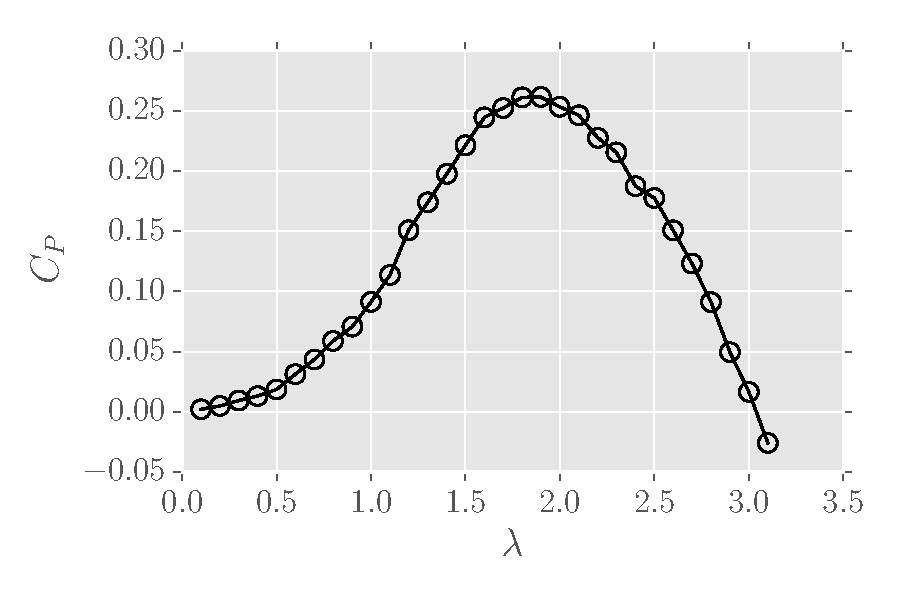
\includegraphics[width=0.65\textwidth]{Figures/cp_vs_tsr.pdf}
\caption{Example of a turbine performance curve.}
\label{fig-cp}
\end{figure}

\begin{figure}[ht]
\centering
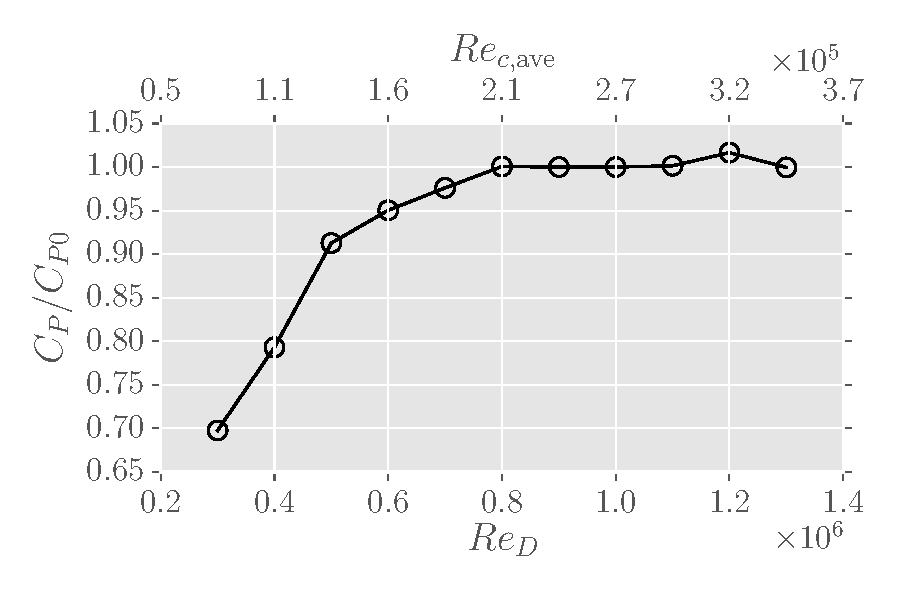
\includegraphics[width=0.65\textwidth]{Figures/re_dep_cp.pdf}
\caption{Normalized turbine power coefficient plotted versus Reynolds number, from \cite{Bachant2014}.}
\label{fig-cp_re_dep}
\end{figure}

\section{Facility and instrumentation}

Experiments will be performed in the UNH tow/wave tank, a 36 m long facility
with a 3.66 m wide by 2.44 m deep cross-section, pictured in
Figure~\ref{fig-tow_tank}. The turbine will be mounted in a frame built from
NACA 0020 struts, attached to the tow carriage by four linear bearings, which
transfer all streamwise force to a pair of S-beam load cells. The turbine shaft
RPM will be controlled by a servo motor system, which allows prescription of the
turbine tip speed ratio. The load torque will be measured by an inline rotary
torque transducer and a load cell mounted at a fixed distance from the servo
motor, providing a redundant measurement. Turbine shaft angle will be measured
using the servo drive's emulated encoder output, set to $10^5$ counts per
turbine shaft revolution. Carriage speed, and therefore inflow velocity will be
measured using a linear encoder with 10 $\mu$m resolution. Turbine wake
measurements at 1 turbine diameter downstream will be measured with a Nortek
Vectrino+ acoustic Doppler velocimeter, sampling at 200 Hz. A list of the
sensors to be used in the experiment is shown in Table~\ref{tab-sensors},
instrumentation in Table~\ref{tab-instrumentation}, and a drawing of the
experimental setup is shown in Figure~\ref{fig-exp_setup}.


\begin{figure}[ht!]
\centering 
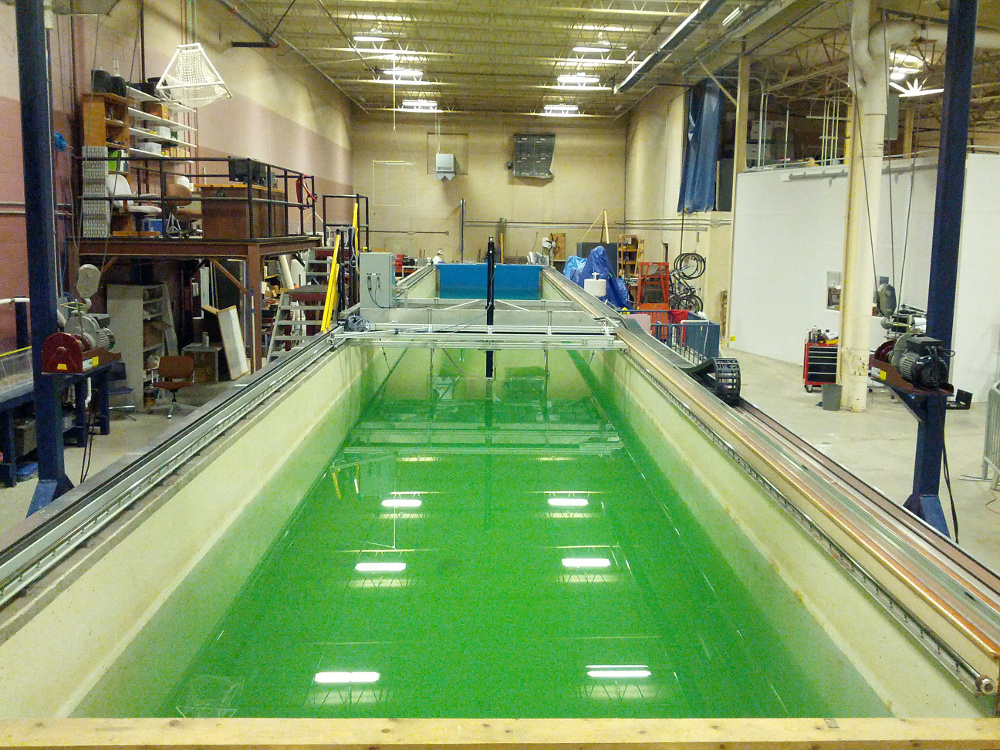
\includegraphics[clip,trim=0 0.4in 0 0.37in, 
width=0.49\textwidth]{Figures/tow_tank_length} 
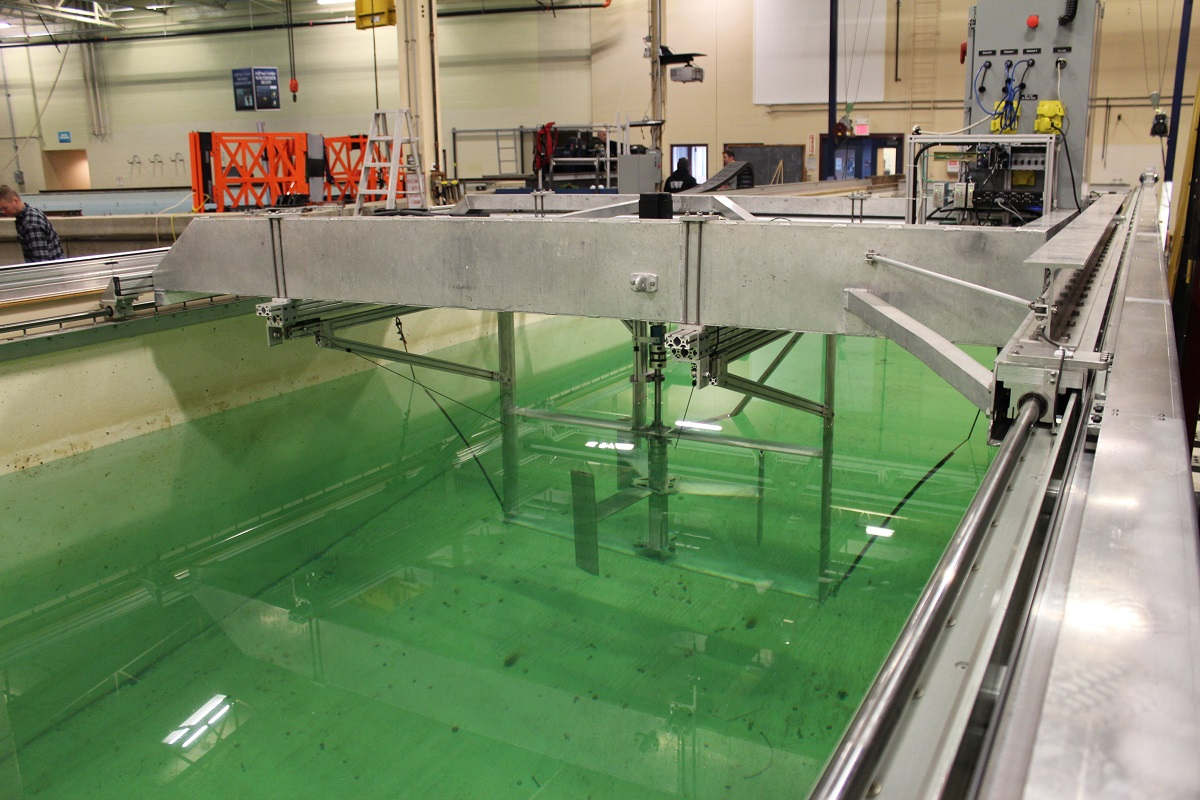
\includegraphics[clip,trim=0.67in 0 0 0, 
width=0.49\textwidth]{Figures/test_bed_photo} 
\caption{Photos of the UNH towing tank and turbine test bed.} 
\label{fig-tow_tank}
\end{figure}


\begin{table}[ht]
\centering
\begin{tabular}{c|c|c|c}
Measured quantity & Device type & Mfg. \& model & Accuracy \\
\hline 
Carriage position & Linear encoder & Renishaw LM15 & 10 $\mu$m/pulse \\
Turbine angle & Drive encoder output & Kollmorgen AKD & 10$^5$ pulse/rev \\
Turbine torque & Rotary transducer & Interface T8-200 & $\pm$0.5 Nm \\ 
Turbine torque (2) & Load cell (\& arm) & Sentran ZB3-200 & $\pm$0.2 Nm \\
Drag force, left & Load cell & Sentran ZB3-500 & $\pm$0.6 N \\
Drag force, right & Load cell & Sentran ZB3-500 & $\pm$0.6 N \\
Fluid velocity & ADV & Nortek Vectrino+ & $\pm$0.5\% $\pm$1 mm/s \\
\end{tabular}
\caption{Details of the sensors to be used for the experiment. Note that ``(2)''
denotes a secondary redundant measurement.} 
\label{tab-sensors}
\end{table}

\begin{table}[ht]
\centering
\begin{tabular}{c|c|c}
Measured quantity & Device type & Mfg. \& model \\
\hline 
Carriage position & Differential counter & NI 9411 \\
Carriage velocity (2) & Motion controller & ACS NTM \\
Turbine angle & Differential counter & NI 9411 \\
Turbine RPM (2) & Motion controller & ACS NTM \\
Turbine torque & Analog voltage input & NI 9405 \\ 
Turbine torque (2) & Analog bridge input & NI 9237 \\
Drag force, left & Analog bridge input & NI 9237 \\
Drag force, right & Analog bridge input & NI 9237 \\
\end{tabular}
\caption{Details of the instrumentation to be used for the experiment. Note that
``(2)'' denotes a secondary redundant measurement.}
\label{tab-instrumentation}
\end{table}

\begin{figure}[ht]
\centering
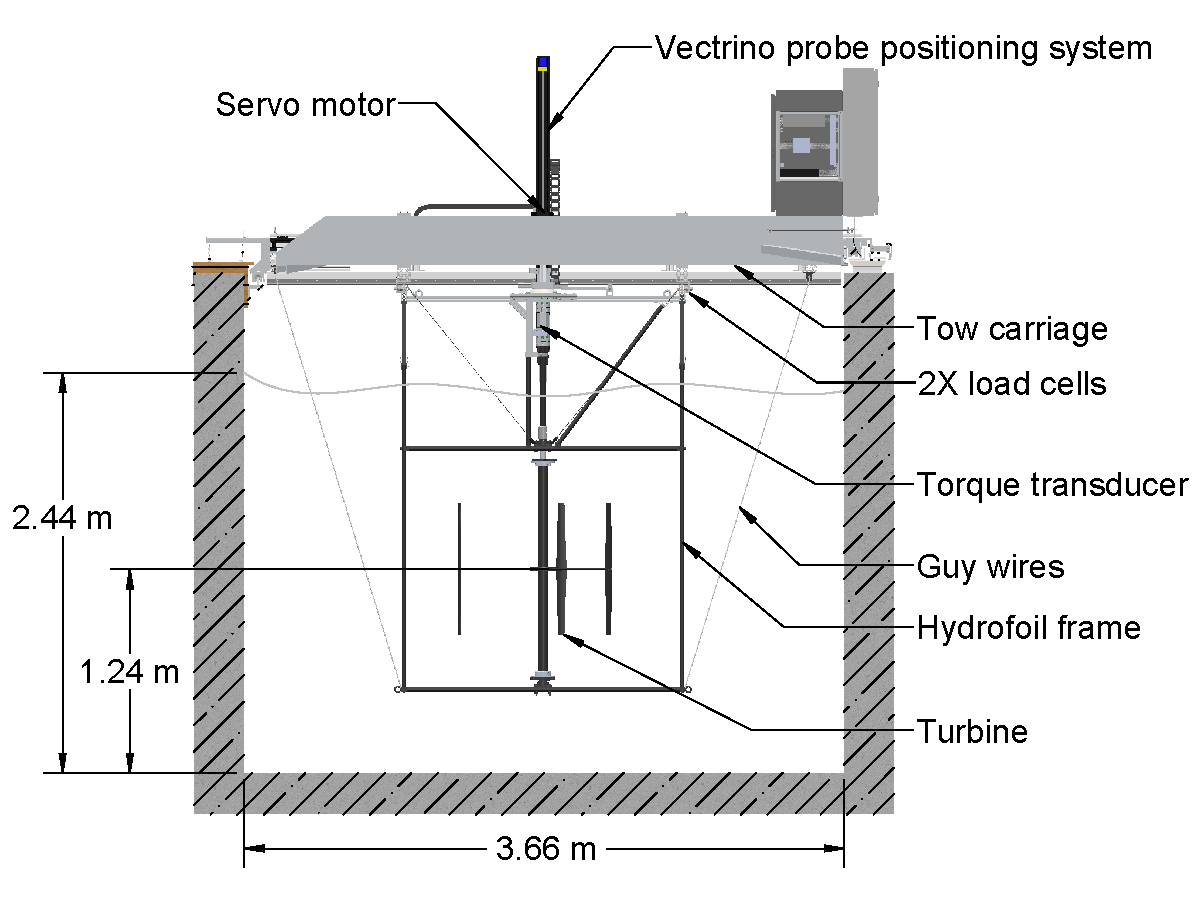
\includegraphics[clip,trim=0.01in 0 0 0, width=0.95\textwidth]{Figures/tank_cross_section}
\caption{Illustration of the experimental setup.}
\label{fig-exp_setup}
\end{figure}


\subsection{Calibrations}

Before collecting data, traceable calibration certificates will be obtained for
the Interface T8-200 torque transducer and NI 9405 and NI 9237 modules. The
torque transducer calibration will be used directly in data processing, while
the load cells will be calibrated using an additional Sentran ZB S-beam load
cell and indicator, a package which will also have its own calibration
certificate. The redundant torque measurement load cell/arm system will also be
calibrated using the Sentran load cell and indicator, attached to a fixture with
a distance from the axis of rotation known to within approximately 0.005 inches.

\subsection{Synchronization of instrumentation subsystems}

The three data acquisition instrumentation subsystems---motion controller, NI
DAQ (performance measurements), and Vectrino+ (wake velocity
measurements)---will begin sampling at precisely the same time each run, after
being triggered by a TTL pulse created by the motion controller. This strategy
retains synchronization for all performance signal samples (tow speed, torque,
drag, angular velocity), ensuring precise calculation of, e.g., power
coefficient. Since there is also synchronization of the initial sample from each
three subsystems, correlation of events in the performance and wake signals is
also possible.

\subsection{Tare drag and torque compensation} 

Tare torque and drag runs will also be performed to measure the shaft bearing
friction torque and turbine mounting frame drag, respectively. These data will
be similar to the turbine performance data, omitting torque measurements for the
tare drag runs and vice versa.

\section{Turbine model}

The turbine is to be a 1:6 scale model of the DOE RM2 rotor, reproduced as
faithfully as possible. Turbine geometry is to be scaled from the RM2 ``rev 0''
design report \cite{Barone2011}, with the exception of the shaft diameter, which
will be a scaled version of the SAFL RM2 shaft \cite{Hill2014}. The hub design
is also similar to the SAFL model, which may aid in comparison of the results,
though this is not a top priority. Geometric parameters are shown in
Table~\ref{tab-turb_geom} and a drawing of the turbine design is shown in
Figure~\ref{fig-turbine_drawing}. 

\begin{table}[ht]
\centering
\begin{tabular}{l|l|l}
   & Full-scale & Model (1:6) \\
\hline 
Diameter (m)   & 6.450 & 1.075 \\ 
Height (m)     & 4.840 & 0.8067 \\ 
Blade root chord (m) & 0.4000 & 0.06667 \\ 
Blade tip chord (m)  & 0.2400 & 0.04000 \\ 
Blade profile & NACA 0021 & NACA 0021 \\ 
Blade mount & 1/2 chord & 1/2 chord \\ 
Blade pitch (deg.) & 0.0 & 0.0 \\ 
Strut profile & NACA 0021 & NACA 0021 \\ 
Strut chord (m) & 0.3600 & 0.06000 \\ 
Shaft diameter (m) & 0.2540 \cite{Beam2011} or 0.4160 \cite{Hill2014} & 0.06350\\ 
\end{tabular}
\caption{RM2 turbine geometric parameters.}
\label{tab-turb_geom}
\end{table}

\begin{figure}[ht]
\centering
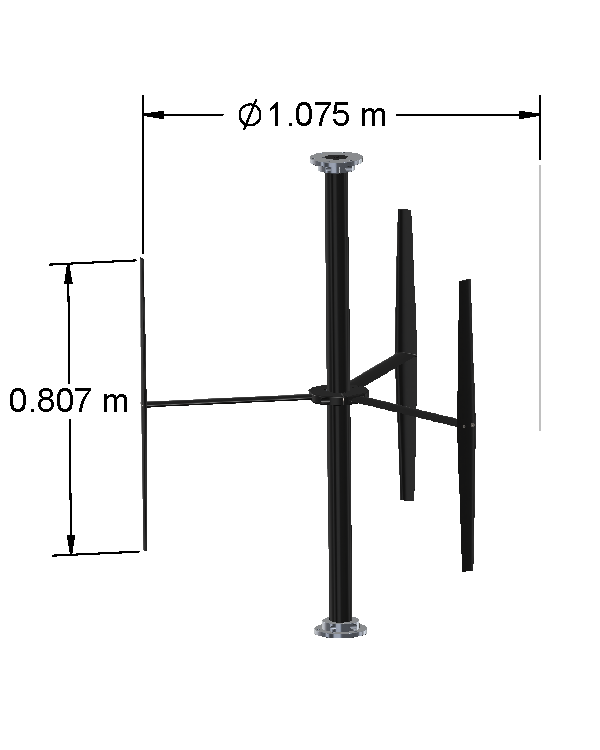
\includegraphics[width=0.5\textwidth]{Figures/turbine}
\caption{Illustration of the UNH RM2 scaled physical model.}
\label{fig-turbine_drawing}
\end{figure}


\section{Test parameters}

Data collection runs will take place during individual tows, for which all
independent variables---tow speed, tip speed ratio, velocity probe
position---are held constant. These runs can then be grouped into logical
``sections,'' in which typically a single independent variable is varied. For
example, a test section will be dedicated to collecting turbine performance
curves for a single tow speed, or turbine diameter Reynolds number, where only
tip speed ratio is varied. An example is shown in Table~\ref{tab-test_section}.
Note that the upper limit of tip speed ratio will be determined in ``shakedown''
runs, and chosen to be just above the value at which turbine power coefficient
reaches zero. Additional performance curve test sections are created/executed
for different tow speeds. For wake characterization, sections will vary the
cross-stream position of the velocity probe, providing a single profile.
Multiple cross-stream profiles would be taken at varying vertical locations,
each of which would represent a test section.

Parameters for each test section will be created in the \texttt{Config/Test
plan} folder inside the experiment working directory, saved in CSV format as
input to the
\textit{TurbineDAQ}\footnote{\url{https://github.com/petebachant/TurbineDAQ}}
experiment automation software. These CSVs also provide information about each
run to be used in post-processing. Note that the software is designed to read
turbine properties (from \texttt{Config/turbine\_properties.json}), e.g. radius
and height, so inputs for turbine rotational speed (tip speed ratio) and
Vectrino probe location are in nondimensional form.


\section{Determining tank settling time}

Sample tows will be done to determine the amount of time taken between runs such
that the tank has settled adequately, i.e., background turbulence and any large
scale mean flows have been dissipated. The settling times will be stored in the
experiment configuration---one value for each tow speed.


\section{Determining Reynolds number independence}

In order to establish that we have reached a Reynolds number independent regime
for turbine performance, we will acquire multiple performance curves, starting
at a tow speed of 0.4 m/s, incrementing by 0.2 m/s, until
convergence is seen in the measured power coefficient. This will be determined
by post-processing the data concurrently.


\section{Measuring the effects of strut drag}

\todo[inline]{Add this.}

\begin{figure}[!ht]
\centering
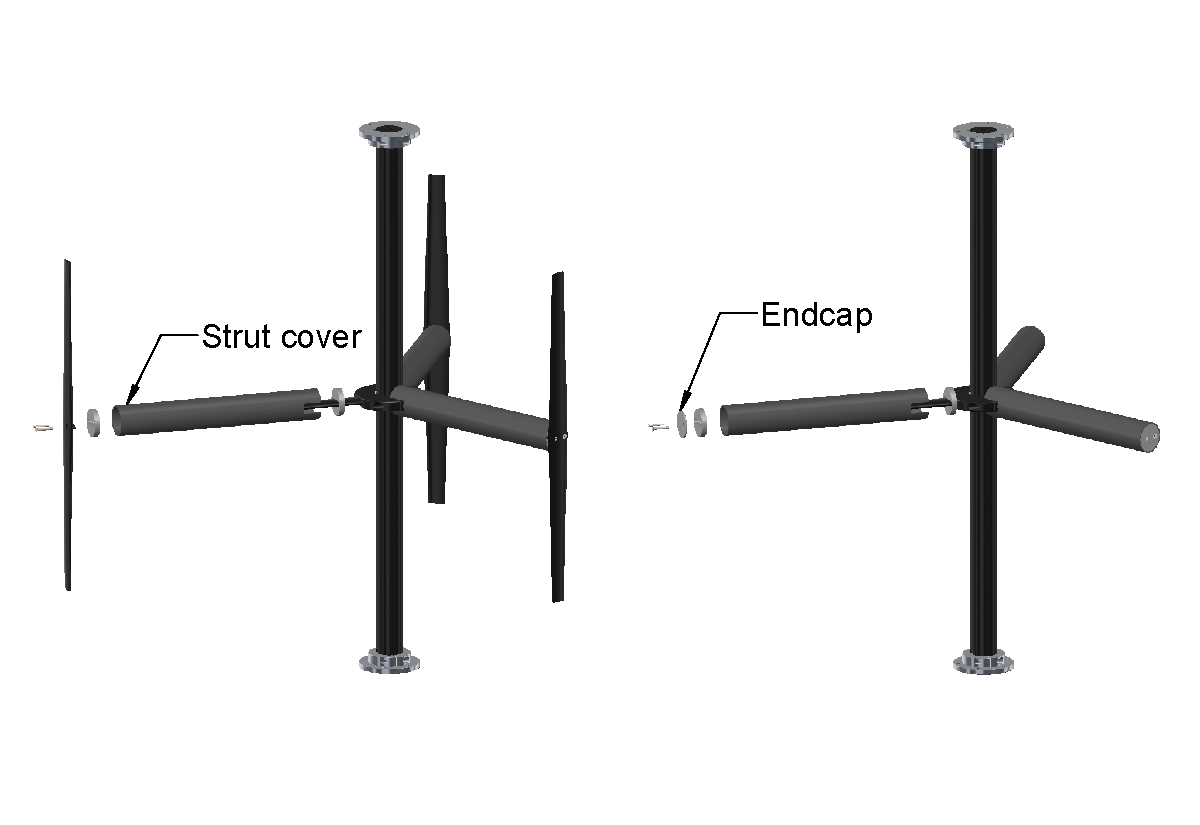
\includegraphics[width=0.8\textwidth]{Figures/strut_covers}
\caption{Illustration of strut cover design with (left) and without (right)
blades installed.}
\label{fig-strut_covers}
\end{figure}

\section{Near-wake characterization}

After Reynolds number independence has been found, we will perform a
characterization of the near-wake at one turbine diameter downstream, acquiring
a series of cross-stream profiles at varying height. The Vectrino will be in a
fixed location for each run, necessitating multiple runs to vary its
cross-stream and vertical coordinates $y/R = \pm 3$ and $z/H = 0$--$0.75$,
respectively. Measurements at these locations will help to visualize the complex
three-dimensional flow field present in the near-wake.

\section{Data processing}

Turbine shaft angular velocity and carriage speed must be computed by taking the
derivatives of the measured position time series. This will be done using a
second order central difference scheme, and may be subsequently filtered with a
moving average filter to help reduce noise introduced by the differentiation. To
check that excess high frequency energy was not removed during filtering, the
velocity signals can be compared to their redundant measurements recorded from
the motion controller.

After the velocity time series are calculated, they are used to calculate time
series for instantaneous $\lambda$, $C_P$, and $C_D$, from which mean values are
computed.

Data collected for each run will include a transient period, where the tow
carriage accelerates, after which turbine torque and wake velocities settle to
become stationary or periodic. It is this ``steady-state'' duration that we are
interested in. The duration will be indentified for several runs at each tow
speed by manual inspection. The tail end will then be truncated such that the
data to be processed includes an integer number of blade passages, to minimize
bias from periodicity. The time interval will be recorded as part of the reduced
data for each run, along with the number of blade passages and revolutions.

Wake velocity data will be post-processed using methods outlined in Gunawan et
al. \cite{Gunawan2011}. Corrections will include, for example, eliminating
and/or replacing spikes \cite{Goring2002}, Doppler noise \cite{Voulgaris1998},
and filtering \cite{Garcia2005}.

\subsection{Uncertainty analysis}

As mentioned previously, one of the primary uses for the data collected is
comparison with results from numerical modeling, and this comparison requires an
estimate for what range of values from the experimental result includes the true
value. This range---or uncertainty---results from a combination of systematic
and random errors. The random error can be inferred from
the sample standard deviation and the systematic from the sensor calibrations or
datasheets. Combining both sources of error, along with their propagation into quantities derived from multiple measurements, will follow the procedures outlined in Coleman and Steele (2009) \cite{ColemanSteele}.

\todo[inline]{Write more about uncertainty analysis.}


\chapter{Research products}

\section{CAD data}

Computer aided design (CAD) data for the turbine model will be provided as both
STEP format 3-D models and 2-D PDFs of the manufacturing drawings.

\section{Experimental data}

A full performance curve for the turbine will consist of 20--30 tows at varying
tip speed ratio. Each of these tows will produce raw data for the turbine
torque, drag force on the submerged equipment, turbine shaft angle, carriage
speed, and Vectrino velocity measurements. Raw data files will be saved from the
NI data acquisition devices at a sample sate of 2 kHz, from the motion
controller at 1 kHz, and from the Vectrino at 200 Hz. All three devices will be
triggered by the motion controller at the beginning of each run so that they
begin sampling at the exact same time.

Raw data will be stored in HDF5 format, run metadata in text-based JavaScript
Object Notation (JSON), processed data in comma separated value (CSV), and
processing code in Python. These formats were chosen for their platform- and
language-independence, which will allow broadest usage of the data by other
researchers. A summary of data file types and names is presented in
Table~\ref{tab-data_description}.


\subsection{Directory structure and naming conventions}

A sample directory structure is shown in Figure~\ref{fig-dir_structure}. In the
\texttt{Config/Test plan} folder are the CSV files containing the test parameter
matrices for each test section. Section names are inferred from the CSV file
names. Raw data files are stored in the \texttt{Data/Raw/\{section\}/\{run\}}
subfolders, while processed data from each section are stored in the
\texttt{Data/Processed} subfolder---one CSV file per experiment section.

\subsection{Metadata}

Metadata recorded for each run will include:

\begin{itemize}

	\item Nominal tow speed
	
	\item Prescribed tip speed ratio
	
	\item Run section and number, e.g., \texttt{"Perf-0.8 run 4"}
	
	\item Time created
	
	\item Turbine name, radius, and height
	
	\item \textit{TurbineDAQ} software version
	
	\item Vectrino location
	
	\item Vectrino metadata
	
		\begin{itemize}
		
			\item Coordinate system
			
			\item Sample rate
			
			\item Velocity range index
		
		\end{itemize}
		
	\item NI device channel metadata
	
		\begin{itemize}
		
		\item Sample rate
		
		\item Scale names, slopes, $y$-intercepts, and units 
		
		\end{itemize}

\end{itemize}


\section{Management and archiving}

This experiment will produce $\sim 10$ GB of data. The two guiding principles
for the management of this data are openness and usefulness, i.e., we want
potential users to know exactly how the data was created, and be able to reuse
the data as conveniently as possible. We will make available all raw and
processed data, along with any software written for the processing, analysis,
and visualization of this data. It is also important that we provide the data
and code such that they are maintainable, both by ourselves and by other users.

Since the dataset is of moderate size, we want to allow users to first
obtain the software and processed data, since these are of most interest for
generating figures or comparing to numerical modeling results. However, if users
want to reanalyze the raw data, the software will be written such that raw data
files are downloaded as needed, rather than one bulk download.

Raw data files will be uploaded to figshare\footnote{\url{http://figshare.com}},
which will then give the dataset a Digital Object Identifier (DOI) and therefore
a persistent URL. Processed data and processing code will be hosted on
GitHub\footnote{\url{https://github.com/UNH-CORE/RM2-tow-tank}} to help
facilitate updates to the analysis by both the investigators and third parties.
This processing code will be written such that raw data is downloaded
automatically as needed. Tagged versions or ``releases'' of the Git repository
will be uploaded to figshare such that they will have their own DOIs, and can be
cited appropriately in publications.

\section{Licensing} 

All research products---documentation, data, code, CAD models, etc.---will be
freely available under a Creative Commons Attribution 4.0 International license,
which allows further sharing and adaptation so long as the original source is
credited.


\chapter{Summary}

\todo[inline]{Write a summary, including a list of explicit research
deliverables.}


\chapter{Acknowledgements}

\todo[inline]{Add these.}


\renewcommand{\bibname}{References}
\bibliography{library}
\bibliographystyle{ieeetr}

\begin{appendices}

\chapter{Sample test plan matrices}

\begin{table}[!ht]
\centering
\scalebox{0.7}{
\begin{tabular}{c|c|c|c|c}
Run & $U_\infty$ & $\lambda$ & $y/R$ & $z/H$ \\
\hline
0 & 1.0 & 0.2 & 0.0 & 0.0 \\
1 & 1.0 & 0.4 & 0.0 & 0.0 \\
2 & 1.0 & 0.6 & 0.0 & 0.0 \\
3 & 1.0 & 0.8 & 0.0 & 0.0 \\
4 & 1.0 & 1.0 & 0.0 & 0.0 \\
5 & 1.0 & 1.2 & 0.0 & 0.0 \\
6 & 1.0 & 1.4 & 0.0 & 0.0 \\
7 & 1.0 & 1.6 & 0.0 & 0.0 \\
8 & 1.0 & 1.8 & 0.0 & 0.0 \\
9 & 1.0 & 2.0 & 0.0 & 0.0 \\
10 & 1.0 & 2.2 & 0.0 & 0.0 \\
11 & 1.0 & 2.4 & 0.0 & 0.0 \\
12 & 1.0 & 2.6 & 0.0 & 0.0 \\
13 & 1.0 & 2.8 & 0.0 & 0.0 \\
14 & 1.0 & 3.0 & 0.0 & 0.0 \\
15 & 1.0 & 3.2 & 0.0 & 0.0 \\
16 & 1.0 & 3.4 & 0.0 & 0.0 \\
17 & 1.0 & 3.6 & 0.0 & 0.0 \\
18 & 1.0 & 3.8 & 0.0 & 0.0 \\
19 & 1.0 & 4.0 & 0.0 & 0.0 
\end{tabular}}
\hspace{0.75in}
\scalebox{0.7}{
\begin{tabular}{c|c|c|c|c}
Run & $U_\infty$ & $\lambda$ & $y/R$   & $z/H$ \\
\hline
0   & $U_0$        & $\lambda_0$ & -3    & 0   \\
1   & $U_0$        & $\lambda_0$ & -2.75 & 0   \\
2   & $U_0$        & $\lambda_0$ & -2.5  & 0   \\
3   & $U_0$        & $\lambda_0$ & -2.25 & 0   \\
4   & $U_0$        & $\lambda_0$ & -2    & 0   \\
5   & $U_0$        & $\lambda_0$ & -1.8  & 0   \\
6   & $U_0$        & $\lambda_0$ & -1.6  & 0   \\
7   & $U_0$        & $\lambda_0$ & -1.5  & 0   \\
8   & $U_0$        & $\lambda_0$ & -1.4  & 0   \\
9   & $U_0$        & $\lambda_0$ & -1.3  & 0   \\
10  & $U_0$        & $\lambda_0$ & -1.2  & 0   \\
11  & $U_0$        & $\lambda_0$ & -1.1  & 0   \\
12  & $U_0$        & $\lambda_0$ & -1    & 0   \\
13  & $U_0$        & $\lambda_0$ & -0.9  & 0   \\
14  & $U_0$        & $\lambda_0$ & -0.8  & 0   \\
15  & $U_0$        & $\lambda_0$ & -0.7  & 0   \\
16  & $U_0$        & $\lambda_0$ & -0.6  & 0   \\
17  & $U_0$        & $\lambda_0$ & -0.5  & 0   \\
18  & $U_0$        & $\lambda_0$ & -0.4  & 0   \\
19  & $U_0$        & $\lambda_0$ & -0.3  & 0   \\
20  & $U_0$        & $\lambda_0$ & -0.2  & 0   \\
21  & $U_0$        & $\lambda_0$ & -0.1  & 0   \\
22  & $U_0$        & $\lambda_0$ & 0     & 0   \\
23  & $U_0$        & $\lambda_0$ & 0.1   & 0   \\
24  & $U_0$        & $\lambda_0$ & 0.2   & 0   \\
25  & $U_0$        & $\lambda_0$ & 0.3   & 0   \\
26  & $U_0$        & $\lambda_0$ & 0.4   & 0   \\
27  & $U_0$        & $\lambda_0$ & 0.5   & 0   \\
28  & $U_0$        & $\lambda_0$ & 0.6   & 0   \\
29  & $U_0$        & $\lambda_0$ & 0.7   & 0   \\
30  & $U_0$        & $\lambda_0$ & 0.8   & 0   \\
31  & $U_0$        & $\lambda_0$ & 0.9   & 0   \\
32  & $U_0$        & $\lambda_0$ & 1     & 0   \\
33  & $U_0$        & $\lambda_0$ & 1.1   & 0   \\
34  & $U_0$        & $\lambda_0$ & 1.2   & 0   \\
35  & $U_0$        & $\lambda_0$ & 1.3   & 0   \\
36  & $U_0$        & $\lambda_0$ & 1.4   & 0   \\
37  & $U_0$        & $\lambda_0$ & 1.5   & 0   \\
38  & $U_0$        & $\lambda_0$ & 1.6   & 0   \\
39  & $U_0$        & $\lambda_0$ & 1.8   & 0   \\
40  & $U_0$        & $\lambda_0$ & 2     & 0   \\
41  & $U_0$        & $\lambda_0$ & 2.25  & 0   \\
42  & $U_0$        & $\lambda_0$ & 2.5   & 0   \\
43  & $U_0$        & $\lambda_0$ & 2.75  & 0   \\
44  & $U_0$        & $\lambda_0$ & 3     & 0  
\end{tabular}}
\caption{Sample test matrices for acquiring a performance curve (left) and a
cross-stream wake profile (right). $U_0$ is a constant a tow speed at which
performance has reached Reynolds number independence, and $\lambda_0$ is the tip
speed ratio at which turbine power coefficient is maximum.}
\label{tab-test_section}
\end{table}


\chapter{Data file organization and content}

\begin{figure}
\begin{verbatim}
RM2-tow-tank/
    Config/
        Test plan/
            Top level.csv
            Perf-0.8.csv
            Wake-U_1.0-zH_0.25.csv
            Tare_drag.csv
            Tare_torque.csv
            Settling.csv
        turbine_properties.json
        settling_times.csv
        raw_data_urls.json
    Data/
        Processed/
            Perf-0.8.csv
            Tare_drag.csv
        Raw/
            Perf-0.8/
                0/
                    metadata.json
                    acsdata.h5
                    nidata.h5
                    vecdata.h5
                    vecdata.vno
                1/    
                    metadata.json
                    acsdata.h5
                    nidata.h5
                    vecdata.h5
                    vecdata.vno
            Tare_drag/
                0/
                    metadata.json
                    acsdata.h5
                    nidata.h5
\end{verbatim}
\caption{Sample directory structure for experiment configuration and data.}
\label{fig-dir_structure}
\end{figure}

\begin{table}[ht]
\centering
\begin{tabular}{l|l|l|l}
Data & Sample rate & File type & File name \\
\hline 
\begin{tabular}[t]{@{}l@{}}
\texttt{time} \\
\texttt{carriage\_pos} \\
\texttt{turbine\_angle} \\
\texttt{torque\_trans} \\
\texttt{torque\_arm} \\
\texttt{drag\_left} \\
\texttt{drag\_right}
\end{tabular} & 2 kHz & HDF5 & \texttt{nidata.h5} \\ 
\hline
\begin{tabular}[t]{@{}l@{}}
\texttt{time} \\
\texttt{carriage\_vel} \\
\texttt{turbine\_rpm} \\
\end{tabular} & 1 kHz & HDF5 & \texttt{acsdata.h5} \\ 
\hline
\begin{tabular}[t]{@{}l@{}}
\texttt{time} \\
\texttt{u} \\
\texttt{v} \\
\texttt{w} \\
\texttt{corr\_u} \\
\texttt{corr\_v} \\
\texttt{corr\_w} \\
\texttt{snr\_u} \\
\texttt{snr\_v} \\
\texttt{snr\_w}
\end{tabular} & 200 Hz & HDF5 & \texttt{vecdata.h5} \\ 
\hline
\begin{tabular}[t]{@{}l@{}}
\texttt{vecdata.dat} \\
\texttt{vecdata.hdr} \\
\texttt{vecdata.pck} \\
\end{tabular} & 200 Hz & Vectrino binary & \texttt{vecdata.vno} \\ 

\end{tabular}
\caption{Raw data file description.}
\label{tab-data_description}
\end{table}

\end{appendices}

\end{document}